% !TEX root = main.tex
\section{Routing a otra Subred}

\begin{figure}[h!]
    \centering
    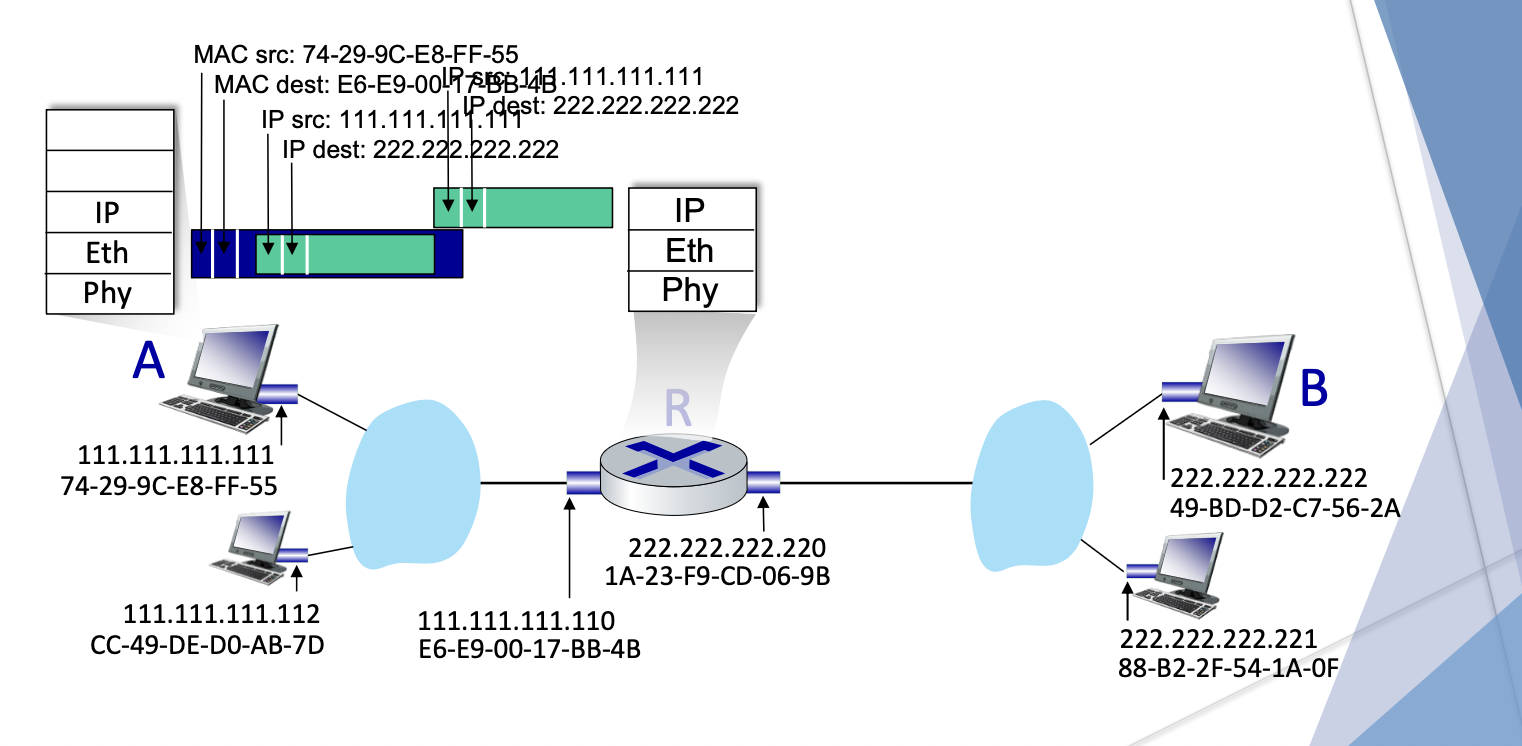
\includegraphics[width=0.5\textwidth]{routing}
    \label{fig:routing}
\end{figure}

\section{Fundamentos de switching}
\subsection{Switches}
Un switch ethernet de capa 2 utiliza solamente las direcciones MAC para tomar decisiones reenvio. Un switch consulta una tabla de direcciones MAC para tomar una decisión de reencío para cada trama.

\subsection{Configuraciones de lso switches}
\begin{enumerate}
\item switches de configuración fija: las caracteristicas y opciones se limitan a las que vienen originalmente con el switch.
\item switches de configuración apilable: se conectan mediante un cable especial, funcionan eficazmente como si fuera un switch grande.
\item switches de configuración modular: el bastidor admite tarjetas de linea que contienen puertos.
\end{enumerate}

\subsection{Switches vs routers}

\begin{figure}[h!]
    \centering
    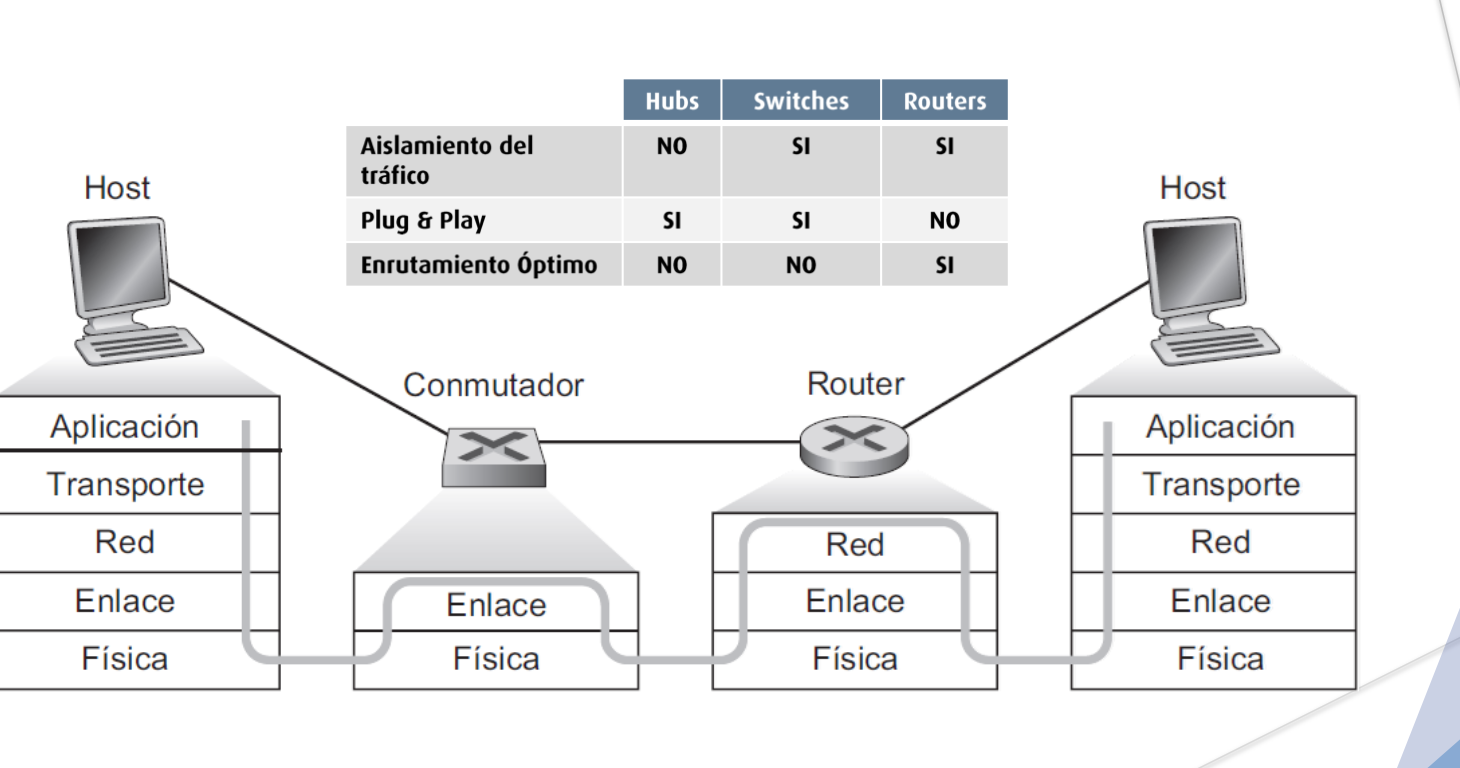
\includegraphics[width=0.5\textwidth]{comparacion}
    \label{fig:comparacion}
\end{figure}

\subsection{Redes de área local virtuales (VLAN)}
Falta de aislamiento del trafico, uso ineficiente de los switches y gestión de los usuarios.

La VLAN \textit{Virtual Local Area Network} es un mecanismo de aislamiento de trafico a nivel de switch. Es un método para crear redes lógicas independientes dentro de una misma red física. Usa etiquetas IEEE 802.1q para identificar el trafico y aísla a los usuarios o los servicios según las politicas. Permite la escalabilidad y la reducción del dominio de difusión.

\textbf{Cómo es la configuración y flujo de VLAN?}

\begin{enumerate}
\item el switch etiqueta los paquetes según la VLAN
\item el router inter-VLAN enruta el trafico y aplica politicas(ACLs)
\item este modelo router-on-a-stick es común en redes pequeñas y medianas
\item se recomienda un rango IP diferente para cada VLAN
\end{enumerate}



